\begin{problem}
Find an example of a finitely generated ring extension $R\subset
S$ where $S$ is a Noetherian ring, but $R$ is not.
\end{problem}
\begin{proof}
\end{proof}
\newpage
\begin{problem}
Consider the homomorphism of rings
\begin{center}
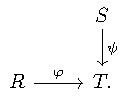
\includegraphics{figures/hw-4-ring-maps}
\end{center}
The \emph{fiber product} of $R$ and $S$ over $T$ is the subring
$R\times_T S=\left\{\,(r,s)\;\middle|\;\phi(t)=\psi(s)\,\right\}$
of $R\times S$. Assume $\phi$ and $\psi$ are surjective. Show
that if $R$ and $S$ are Noetherian rings then so is $R\times_T
S$.
\end{problem}
\begin{proof}
Suppose that $R$ and $S$ are Noetherian rings with surjective
ring maps $\phi\colon R\to T$ and $\psi\colon S\to T$. Then, by
(3.5), the product $R\times S$ is Noetherian. Define the ring map
$\Phi\colon R\times S\to T\times T$ by $\Phi=(\phi,\psi)$. Then
the diagonal, $\Delta_T=\left\{\,(t,t)\;\middle|\; t\in
  T\,\right\}$, of $T\times T$ is exactly the image of the fiber
product of $R$ and $S$ under the ring map $\Phi$. And this is not
terribly difficult to see: It is clear, by the definition of the
fiber product, that $\Phi(R\times_T S)\subset\Delta_T$. To show
the reverse containment, take an element
$(t,t)\in\Delta_T$. Then, since $\phi$ and $\psi$ are surjective,
there are corresponding elements $r$ and $s$ of the rings $R$ and
$S$, respectively, such that $\phi(r)=t$ and $\psi(s)=t$. Hence,
$(t,t)$ are in the image $R\times_T S$ under $\Phi$.

Now, it is clear that $R\times S$ and $T\times T$ have an
$R\times S$-module structure ($R\times S$ by the usual ring
multiplication and $T\times T$ by
$(r,s)(t,t')=(\phi(r)t,\psi(s)t')$) so they have an $R\times_T
S$-module structure by restriction to the subring $R\times_T S$
of $R\times S$. Consider the quotient module $T\times
T/\Delta_T$. $T\times T/\Delta_T$ also inherits an $R\times_T
S$-module structure from $T\times T$. Note that the map
$\Phi\colon R\times S\to T\times T$ is an $R\times_T S$-linear
map: It is clear that $\Phi$ is linear with respect to ``$+$'', what
is not so obvious is that multiplication by scalars is preserved
so take $(r',s')\in R\times_T S$ and $(r,s)\in R\times S$, then
\begin{align*}
\Phi((r',s')(r,s)&=
\Phi(r'r,s's)\\
&=(\phi(r'r),\psi(s's'))\\
&=(\phi(r')\phi(r),\psi(s')\psi(s))\\
&=(\phi(r'),\psi(s'))(\phi(r),\psi(s))\\
&=\Phi(r',s')\Phi(s,r)
\end{align*}
as desired. Therefore, $\Phi$ induces an $R\times_T S$-linear map
$\Phi^*\colon R\times S\to T\times T/\Delta_T$ via composition
with the quotient map, i.e., $\Phi^*=\pi\circ\Phi$ and we have
the following exact sequence of $R\times_T S$-modules
\begin{center}
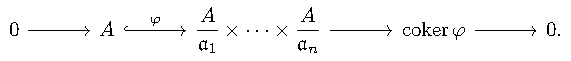
\includegraphics{figures/ps4-p2-short-exact-seq}
\end{center}
By (3.4), $R\times_T S$ are Noetherian.
\end{proof}
\newpage
\begin{problem}
Let $M$ be an $R$-module. Show that $M$ is a flat $R$-module if
and only if $M_{\mathfrak{m}}$ is a flat
$R_{\mathfrak{m}}$-module for every maximal ideal $\mathfrak{m}$
of $R$.
\end{problem}
\begin{proof}
$\implies$: Suppose that $M$ is a flat $R$-module.

$\impliedby$:
\end{proof}
\newpage
\begin{problem}
Let $M$ be an $R$-module and $\mathfrak{a}$ an $R$-ideal.
\begin{enumerate}[noitemsep,label=(\alph*)]
\item Show that if $M_{\mathfrak{m}}=0$ for every maximal ideal
  $\mathfrak{m}$ containing $\mathfrak{a}$, then $M=\mathfrak{a}M$.
\item Show that the converse holds in case $M$ is finite.
\end{enumerate}
\end{problem}
\begin{proof}
(a) Suppose that $M_{\mathfrak{m}}$ for every maximal ideal
$\mathfrak{m}$ containing $\mathfrak{a}$.
\end{proof}
\newpage
\begin{problem}
Prove that every power of a maximal ideal is primary.
\end{problem}
\begin{proof}
\end{proof}
\newpage
\begin{problem}
\begin{enumerate}[noitemsep,label=(\alph*)]
\item Show that the radical of a primary ideal is prime.
\item Find an example of a power of a prime ideal that is not
  primary.
\item Let $\mathfrak{p}$ be a prime ideal of a ring $R$ and
  $n\in\NN$. The $R$-ideal
  $\mathfrak{p}^{(n)}=R\cap\mathfrak{p}^nR_{\mathfrak{p}}$ s
  called the \emph{$n$th symbolic power of $\mathfrak{p}$}. Show
  that $\mathfrak{p}^{(n)}$ is primary.
\end{enumerate}
\end{problem}
\begin{proof}
\end{proof}

%%% Local Variables:
%%% mode: latex
%%% TeX-master: "../MA557-HW-Current"
%%% End:
